\documentclass[11pt, a4paper]{article}
\usepackage[style=script-v1, privacy=anonym]{../tools/library}
\renewcommand{\Lecturer}{Prof. A. Thom, Dr. V. Alekseev}
\begin{document}

\head{AL10: Algebra I}{Wintersemester 2025/2026}
\tableofcontents

\newpage


\section{Multilineare Algebra}
\subsection{Tensorprodukte}

\begin{definition} \Xlabel{Definition}{subsub}{Tensorprodukt}
    Seien $V,W$ $\K-$Vektorräume. Ein Vektorraum $T$ zusammen mit einer
bilinearen Abbildung $\beta: V \times W \to T$ heißt \emph{Tensorprodukt} von $V$ und $W$, wenn $T$ folgende
universelle Eigenschaft besitzt: Für jeden $\K-$Vektorraum $Z$ und jede bilineare Abbildung $\varphi: V\times W \to Z$ existiert eine eindeutige lineare Abbildung $\Bar{\varphi}: T\to Z$ mit $\Bar{\varphi}\circ \beta = \varphi:$


\begin{figure}[h]
    \centering
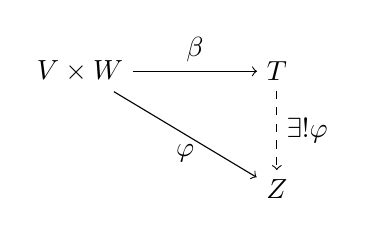
\begin{tikzpicture}[node distance=1cm, auto]

\node (VW) at (0,0) {$V \times W$};
  \node (tensor) at (2.5,0) {$T$};
  \node (X) at (2.5,-1.5) {$Z$};

\draw[->] (VW) -- (tensor) node[midway, above] {$\beta$};
  \draw[->] (VW) -- (X) node[midway, below] {$\varphi$};
  \draw[->, dashed] (tensor) -- (X) node[midway, right] {$\exists! \Bar\varphi$};

\end{tikzpicture}
\end{figure}

Wir bezeichnen $T:= V\otimes W$
\end{definition}

\begin{lemma}[Eindeutigkeit des Tensorprodukts] Falls $T:=V\otimes W$ existiert, dann ist dieses Tensorprodukt eindeutig (bis auf eindeutige Isomorphie). Dies folgt direkt aus der universellen Eigenschaft.
\end{lemma}

\begin{definition}\Xlabel{Definition}{subsub}{Freier Vektorraum}
    Sei $S$ eine beliebige Menge. Wir definieren
    $$\mathcal F (S) := \bigoplus_{s\in S} \K = \{(a_s)_{s\in S} |a_s = 0 \text{ für fast alle $s\in S$}\}$$
    als den \emph{freien $\K-$Vektorraum über S}.
\end{definition}

\begin{lemma}[Existenz des Tensorprodukts]
    Das Tensorprodukt $V\otimes W$ existiert für jedes Paar $V,W$. Die explizite Konstruktion lautet:

    $$V\otimes W:= \mathcal F(V\times W) / I,$$
    wobei $I$ das folgende Ideal sein soll
    $$I:= \left\langle \begin{matrix}
        \lambda (v,w) - (\lambda v, w),\;  \lambda(v,w) - (v,\lambda w), \\
        (v_1 +v_2 , w) -(v_1,w) -(v_2,w),\\ (v, w_1+w_2) -(v,w_1) -(v,w_2)
    \end{matrix} \; \Bigg|\; \begin{matrix}
        v,v_1,v_2\in V \\ w,w_1,w_2 \in W \\ \lambda \in \K 
    \end{matrix} \right\rangle $$
    mit der bilinearen Abbildung $$\beta: V\times W \to V\otimes W,\quad  (v,w)\mapsto [(v,w)]=: v\otimes w$$
\end{lemma}

\begin{note}
    Nach dieser Konstruktion des Tensorproduktes haben wir die folgenden Relationen innerhalb des Tensors von $V\otimes W$ erzwungen:
    \begin{align*}
    \lambda (v\otimes w)&= \lambda v\otimes w = v\otimes \lambda w \\
    (v_1+v_2)\otimes w &= v_1 \otimes w + v_2 \otimes w \\
    v \otimes (w_1+w_2) &= v\otimes w_1 + v\otimes w_2
    \end{align*} 
    Des weiteren existieren natürliche Fortsetzungen des Tensoroperators auf die Vektorräume 
    \begin{enumerate}
        \item $\mathrm{Hom}(V,Z)\otimes \mathrm{Hom}(W,U):$
        $$f\otimes g: V\otimes Z \to W\otimes U, \quad v\otimes w \mapsto f(v) \otimes g(v)$$
        \item $V^*\otimes W^*:$
        $$\alpha \otimes \beta: V\otimes W \to \K, \quad v\otimes w \mapsto \alpha(v)\cdot \beta(w)$$
        \item $\K \otimes \K \cong \K:$
        $$\Phi:\K \otimes \K \to \K,\quad \lambda \otimes \eta \mapsto \lambda \cdot \eta$$
    \end{enumerate}
\end{note}

\begin{lemma}\Xlabel{Lemma}{subsub}{Lineare Unabhängigkeit im Tensorprodukt} Seien $v_1,\dots , v_n \in V$ linear unabhängig, $w_1,\dots , w_n\in W$ beliebig ungleich Null. Dann sind $v_1\otimes w_1, \dots , v_n \otimes w_n$ linear unabhängig in $V\otimes W$.
\end{lemma}
\begin{corollary}[Tensorproduktbasis] Wenn $B= (b_i)_{i\in I}, C=(c_j)_{j\in J}$ Basen in $V$ bzw. $W$ sind, dann ist $B\otimes C:= (b_i \otimes c_j)_{i\in I, j \in J}$ eine Basis von $V\otimes W$
\end{corollary}

\begin{corollary}[Dimension des Tensorprodukts] Falls $V,W$ endlichdimensional, dann gilt:
$$\dim V\otimes W = \dim V \cdot \dim W $$
\end{corollary}

\begin{example}\Xlabel{Beispiele}{subsub}{weitere natürliche Isomorphien}
Es sind die folgenden Tensorprodukte und Vektorräume auf natürliche Weise isomorph zueinander:

\begin{enumerate}
    \item $W\otimes V^* \cong \Hom V W \quad \varphi: W\otimes V^* \to \End{V}, \ w\otimes \alpha \mapsto (v \mapsto \alpha(v)w)$\par
    Hinweis: Es gibt in $V\otimes W$ Elemente, die sich ggf. nicht durch Elementartensoren darstellen lassen. Diese morphen zu Homomorphismen höreren Ranges.
    \item $V\otimes V^* \cong \End{V}, \quad \varphi: V\otimes V^* \to \End V, \ v\otimes \alpha \mapsto (x\mapsto \alpha(x)v)$ 
    \item $\K \otimes \K \cong \K, \quad \varphi: \K \otimes \K \to \K, \lambda \otimes \eta \mapsto \lambda \cdot \eta$
\end{enumerate}

    
\end{example}
\subsection{Äußere Algebra}

\begin{definition} \Xlabel{Definition}{subsub}{Tensoralgebra}
    Sei $V$ ein $\K-$Vektorraum. Die \emph{Tensoralgebra} $T(V)$ ist definiert als
    $$T(V):= \bigoplus _{k = 0}^\infty V^{\otimes k} = \K \oplus V \oplus V\otimes V \oplus...$$
    wobei $V^{\otimes k}= \underbrace{V\otimes \cdots \otimes V}_{k}$ meint.
\end{definition}

\begin{note}
    Die hinzugekommene ``Multiplikation'' meint hier das Nebeneinanderschreiben der Tensoren.
    $$(v_1 \otimes \cdots \otimes v_n) \otimes (w_1 \otimes \cdots w_m) = v_1 \otimes \cdots \otimes v_n \otimes w_1 \otimes \cdots w_m$$
    Diese ist so schon ausreichend definiert, weil $\otimes$ nach Konstruktion bereits bilinear ist. Es benötigt für eine sinnvolle Struktur noch eine Symmetrie-Forderung an diese Tensor-Multiplikation, es genügt allerdings Schiefsymmetrie wie wir sehen werden, um die später noch folgenden gewünschten Objekte besser studieren zu können.
\end{note}

\begin{definition}\Xlabel{Definition}{subsub}{Äußere Algebra} Sei $I_\wedge (V)$ das Ideal definiert durch
$$I_\wedge(V) := \langle v\otimes v | v\in V\rangle\; \triangleleft\;  T(V)$$
Dann bezeichnen wir mit 
$$\Lambda(V):= T(V)/I_\wedge(V)$$
die \emph{äußere Algebra von V}. Wir notieren die Elemente von $\Lambda (V)$ mit 
$$v_1 \wedge \cdots \wedge v_k = [v_1 \otimes \cdots \otimes v_k]_{I_\wedge (V)} \in \Lambda (V)$$
\end{definition}

\begin{note}
    Mit der Definition der äußeren Algebra als Quotienten erzwingen wir die folgenden Eigenschaften:
\begin{align*}
    v\wedge v &= 0\\
    v\wedge w &= - w\wedge v
\end{align*}
denn $\underbrace{(v+w)\wedge (v+w)}_{0} = \underbrace{v\wedge v}_{0} +v\wedge w + w\wedge v +\underbrace{w\wedge w}_{0} = 0$.\\
Entsprechend ist das $\wedge-$Produkt in $\Lambda (V)$ schiefsymmetrisch oder \emph{antikommutativ}.
\end{note}

\begin{definition}[$k$-te äußere Algebra] 
    Wir meinen gerade mit $$\Lambda^k (V):=[V^{\otimes k}]_{I\wedge (V)} \subset \Lambda (V)$$
    den direkten Anteil der äußeren Algebra, der gerade ein Wedgeprodukt aus genau $k$ Vektoren aus $V$ ist. Es gilt daher auf natürliche Weite die äquivalente Definition
    $$\Lambda (V) = \bigoplus_{k=1}^\infty \Lambda^k(V)$$
\end{definition}

\begin{corollary}[Endlichkeit und Dimension der äußeren Algebra]
Betrachte $\Lambda (V)$ über einem endlich-dimensionalen Vektorraum $V$ mit $\dim V= n$. Dann gilt
$$\dim\Lambda(V) = 2^n = 2^{\dim V}$$
\end{corollary}

\begin{corollary}[Dimension der $k$-ten äußeren Algebra] Weil jeweils das geordnete Tupel 
$(b_{i_1} \wedge \cdots \wedge b_{i_k})_{1\leq i_1 < ... < i_k \leq n}$ eine Basis von $\Lambda^k (V)$ bildet, muss
$$\dim \Lambda^k (V) = \binom n k$$
\end{corollary}


\subsection{Alternierende Formen und Determinante}

\begin{definition}[Alternierende multilineare Abb.]
    Eine multilineare Abbildung $\alpha: V^k \to \K$ heißt alternierend, falls
    $$\alpha(v_1,...,v_i,...,v_j,...,v_n)= -\alpha(v_1,...,v_j,...,v_i,...,v_n)$$
    für alle $i\neq j \in \{1,...,n\}$. Wir bezeichnen mit 
    $$A_k(V) := \{\alpha: V^k \to \K \ | \ \alpha \text{ multilinear \& alternierend}\}$$
\end{definition}

\begin{corollary}
    Aufgrund der Schiefsymmentrie des $\wedge-$Produkts entsteht folgende natürliche Isomorphie:
    $$(\Lambda^k V)^* \cong \Lambda^k V^* \cong A_k (V)$$
\end{corollary}

\begin{definition}[Volumenformen] Der Vektorraum $\Lambda^n(V^*)$ mit $n= \dim V^*$ heißt Raum der Determinantenformen. Ein Element $\omega \in \Lambda^n(V^*)\setminus \{0\}$ heißt Volumenform auf $V^*$.
\end{definition}

\begin{definition}[Induzierte Abbildungen auf Tensoralgebren]
    Sei $f\in \Hom V W$. Bezeichne mit 
    $$T(f): T(V) \to T(W), \; v_1\otimes ...\otimes v_n \mapsto f(v_1) \otimes ...\otimes f(v_n) $$
    die durch $f$ auf die Tensoralgebra induzierte multilineare Abbildung. Weiterhin haben wir eine homomorphe Induktion nach $\Lambda(V)$ mit 
    $$\Lambda(f): \Lambda(V) \to \Lambda(W), \; v_1\wedge ...\wedge v_n \mapsto f(v_1) \wedge ...\wedge f(v_n) $$
    und kanonisch in dieser Definition schon inkludiert $\Lambda^k f$. 
\end{definition}

\begin{note}
    Bemerke dass für $V$ endlichdimensional und $\dim V = n$ die Dimension $\dim \Lambda ^n V = 1$ und damit 
    $\Lambda ^n f: \Lambda^n(V) \to \Lambda^n(V)$ eine eindimensionale Abbildung vom Rang höchstens 1 sein kann und damit durch $x\mapsto \alpha x$ mit $\alpha\in \K$ gegeben sein muss. Dieses $\alpha $ ist tatsächlich eindeutig. Es kann nur eine solche Abbildung für jedes $f$ existieren.
\end{note}

\begin{definition}\Xlabel{Definition}{subsub}{Determinante} Sei $V$ $\K-$Vektorraum, $\dim V= n$ und $f\in \End V$. Dann ist $\det f \in \K$ eindeutig bestimmt als dasjenige Skalar, für das die Funktion 
$$\Lambda^n f: \Lambda^n (V) \to \Lambda^n(V), v_1 \wedge ...\wedge v_n \to \det f v_1 \wedge ...\wedge v_n $$
multilinear ist bzw. das Körperelement, für das gilt :
$$\Lambda^n f = \det f \cdot \id_{\Lambda^n V}$$
\end{definition}

\newpage
\section{Gruppentheorie}
\subsection{Grundlagen}
\begin{definition}[Transformationsgruppe]
    Sei $X$ eine beliebige Menge und $G \leqslant\Sym(X)$ eine Untergruppe. Dann heißt $G$ Transformationsgruppe auf $X$
\end{definition}

\begin{definition}[Äquivalenz under Transformationsgruppen]
    Seien $F,F'\subset X$ und $G\leqslant \Sym(X)$. Dann heißen
    $$F,F' \text{ äquivalent unter $G$} :\Longleftrightarrow \exists g\in G \text{ mit } g(F) = F'$$
\end{definition}

\begin{definition}[G-Symmetrien]
Sei $G$ eine Transformationsgruppe auf $X$. Die $G-$Symmetrien von $F\subset X$ sind definiert als
$$\Sym_G(F):= \{g\in G \; | \; g(F) = F\}$$
also diejenigen Transformationen, die $F$ invariant lassen.
\end{definition}

\begin{definition}[Zyklische Untergruppen]
Sei $g\in G$. Dann bezeichnet
$$\langle g \rangle := \{g^k | k \in \Z\}$$
die durch $g$ erzeugte zyklische Untergruppe.
    
\end{definition}

\begin{definition}[Ordnung]
    Sei $g\in G$. Dann ist 
    $$\ord(g):= \inf\{k\in \Z | g^k = 1 \}$$
    die Ordnung von $g$. Wir bezeichnen mit $|G|$ (Anzahl der Elemente von $G$) die Ordnung von $G$ 
\end{definition}

\begin{definition}[Zyklische Gruppen]
Sei $G$ eine Gruppe. Falls $\exists g\in G$ mit $\langle g \rangle = G$, dann heißt $G$ zyklisch. $g$ heißt dann Erzeuger von $G$.
    
\end{definition}

\begin{lemma}[Eigenschaften zyklischer Gruppen]
Sei $G$ eine Gruppe. 
\begin{enumerate}
    \item Falls $G$ zyklisch und unendlich, dann ist $G\cong \Z$, falls endlich, dann $G\cong \Z/n\Z$
    \item $g^k\in \langle g\rangle = G$ ist genau dann ein Erzeuger, wenn $\gcd(n,k)=1$
    \item Jede Untergruppe einer zyklischen Gruppe ist zyklisch. Falls $|G|=n$ und $q\mid n$, dann existiert genau eine Untergruppe $H\leqslant G$ mit $|H|=q$
    \item Falls $|G|=p$ prim, dann ist jede nichttriviale zyklische Untergruppe von $G$ die Gruppe selbst.
\end{enumerate}
\end{lemma}

\begin{definition}\Xlabel{Definition}{subsub}{Erzeugte Untergruppen}
Sei $S\subset G$ eine beliebige Teilmenge einer Gruppe $G$. Dann ist 
$$\langle S \rangle := \bigcap _{S\subset H\leqslant G} H$$
die sogenannte \emph{von $S$ erzeugte Untergruppe}. $G$ wird von $S$ erzeugt, falls $\langle S\rangle = G$
\end{definition}

\subsection{Gruppenwirkungen - Allgemein}
\begin{definition}\Xlabel{Definition}{subsub}{Gruppenwirkung}
Sei $G$ eine Gruppe und $X$ eine Menge.
Eine Wirkung $G \curvearrowright^\alpha X$ ist ein Homomorphismus $$\alpha: G \to \Sym (X), \; g\mapsto \alpha_g$$
Entsprechend bleibt bei einer qualifizierten Abbildung die Homomorphie-Eigenschaft zu überprüfen:
$$\forall g,h \in G \quad \alpha_{g\cdot h} = \alpha_g \circ \alpha_h$$
Ein $G-$Raum ist dann eine Menge $X$ zusammen mit einer festen Wirkung $G\curvearrowright ^\alpha X$. Falls $\alpha$ fixiert bleibt, schreibe $\alpha_g(x)=: g\cdot x$ für $x\in X, g\in G$
\end{definition}

\begin{definition} \Xlabel{Definition}{subsub}{Bahn / Orbit}
    Sei $G \curvearrowright^\alpha X$ eine Wirkung und $x\in X$. Dann bezeichnet
    $$G\cdot x := \{\alpha_g(x) \;| g\in G\}$$
    die \emph{Bahn} oder den \emph{Orbit von $x$}.
\end{definition}

\begin{corollary}[Orbit-Äquivalenzrelation]
    Sei $G \curvearrowright^\alpha X$ eine Wirkung. Die Relation $$x\sim y :\Longleftrightarrow G\cdot x = G\cdot y$$ ist eine Äquivalenzrelation. Wir bezeichnen den Quotienten 
    $$X/_\sim =: G\backslash X$$
    als Bahnenraum oder Quotientenraum der Wirkung. Es gilt auch die triviale Äquivalenz:
    $$x\sim y \Longleftrightarrow \exists h \in G \quad x = h\cdot y$$
\end{corollary}

\begin{lemma} \Xlabel{Lemma}{subsub}{Orbitzerlegung}
Sei $G \curvearrowright^\alpha X$ eine Wirkung. Dann zerlegt sich die Menge $X$ disjunkt in die Orbits der Äquivalenzklassen von $G\backslash X$:

$$X = \bigsqcup _ {[x]\in G\backslash X} G\cdot x$$
    
\end{lemma}

\begin{definition}\Xlabel{Definition}{subsub}{Transitivität}
Eine Wirkung  $G \curvearrowright^\alpha X$ heißt transitiv, falls $\exists x \in X$ mit $G\cdot x = X$.
\end{definition}

\begin{note}\label{Äquivalenz-Transitivität}
    Falls $G \curvearrowright^\alpha X$ eine transitive Wirkung ist, dann gilt die Äquivalenz
    $$\exists x\in X\; G\cdot x = X \Longleftrightarrow \forall x\in X \; G\cdot x = X$$
\end{note}

\begin{note} Per Definition wirkt $G$ auf jede Bahn $G\cdot x$ transitiv. Jede Wirkung ist damit disjunkt zusammengesetzt aus transitiven Wirkungen und wir können unser Studium deshalb auf diese beschränken.
\end{note}

\begin{definition}\Xlabel{Definition}{subsub}{Stabilisator} Sei  $G \curvearrowright^\alpha X$ eine Wirkung und $x\in X$. Dann ist
$$\Stab(x):= \{g\in G|\; \alpha_g(x) = x\}$$
Wir nennen $x$ einen Fixpunkt der Wirkung, falls $\Stab(x) = G$. Offensichtlich ist $\Stab(x)\leqslant G$
\end{definition}

\begin{definition}[G-Äquivarianz] Seien  $G \curvearrowright^\alpha X$ und  $G \curvearrowright^\beta Y$ zwei $G-$Wirkungen. Eine Abbildung $\varphi: X\to Y$ heißt \emph{$G-$äquivariant}, falls 
$$\varphi(\alpha_g(x)) = \beta_g(\varphi(x)) \quad \forall x\in X, g\in G$$
    
\end{definition}
\subsection{Gruppenwirkungen auf Gruppen}
\begin{definition}[Links- und Rechtswirkungen] \label{Links- und Rechtswirkungen}
    Seien $G\curvearrowright^L G$ und $G\curvearrowright^R G$ die Links- bzw. Rechtswirkungen von $G$ auf sich selbst mit $L_g(h):=gh$ und $R_g(h):= hg\r$. Dann können wir diese Wirkung einfach als die abgeschlossene Gruppenoperation sehen und damit die Struktur der Gruppe selbst besser untersuchen.
\end{definition}
\begin{definition}[Nebenklassen]
Sei $H\leqslant G$ Untergruppe. Dann können wir die Wirkungen aus \ref{Links- und Rechtswirkungen} eben so gut einschränken auf $H \curvearrowright G$. Betrachte zunächst $H \curvearrowright^L G$ die \textbf{Links-}Wirkung von $H$. Dann entstehen nach der Orbitzerlegung \ref{Orbitzerlegung} die \textbf{Rechts-}Nebenklassen in ihrem Quotienten, die wir mit
$$Hg := \{hg \in G | \;  h \in H\}\in H\backslash G$$
bezeichnen. Entsprechend entstehen bei der \textbf{Rechts-}Wirkung $H \curvearrowright^R G$ die \textbf{Links-}Nebenklassen
$$gH:= \{gh \in G| \; h\in H\}\in G/H$$
\emph{Hinweis:} Häufig werden die Notationen inkonsistent benutzt. Es gilt jeweils den Quotienten und dessen Nebenklassen immer bezüglich der aktuellen Wirkung zu betrachten.
\end{definition}

\begin{note}
    Für abelsche Gruppen $G$ stimmen Rechts- und Linksnebenklassen überein.
\end{note}


\begin{definition}[Konjugationswirkung]
Die sehr häufig betrachtete Konjugationswirkung $G\curvearrowright^C G$ ist definiert durch $C_g(h)= ghg\r$. Hier betrachtet man wiederrum selten Nebenklassen, sondern eher Untergruppen \textbf{auf die} gewirkt wird. Wir bezeichnen mit
$$gHg\r := \{ghg\r \in G | h\in H\}$$
die durch $g$ zu $H$ konjugierte Untergruppe.
    
\end{definition}

\begin{theorem}[Klassifikation von transitiven Wirkungen] \label{Klassifikation von transitiven Wirkungen}
Sei $G\curvearrowright X$ eine transitive Wirkung und $x\in X$ fest (Bemerke \ref{Äquivalenz-Transitivität}). Dann gilt die folgende Isomorphie:
$$G\curvearrowright X \cong G\curvearrowright G/\Stab(x)$$ mittels des Isomorphimus 
$$\varphi: X\to G/\Stab(x), \quad y = g\cdot x \mapsto [g]_{\Stab(x)}$$
man sieht:
$$\ker \varphi = \{y= g\cdot x\in X | \; g\in \Stab(x) \} = \{x\}$$
$$\varphi\r: G/\Stab(x) \to X, \;[g]_{\Stab(x)} \mapsto g\cdot x$$
alles wohldefiniert.
    
\end{theorem}

\begin{corollary}\Xlabel{Korollar}{subsub}{Klassifikation von Wirkungen}
Sei $G\curvearrowright^\alpha X$ eine Wirkung. Dann besteht ein Isomorphismus:
$$G\curvearrowright X \; \cong \; \bigsqcup _{[x]\in X/G} G\curvearrowright G/\Stab(x)$$
mittels der Konstruktion in \ref{Klassifikation von transitiven Wirkungen}
    
\end{corollary}

\begin{definition}[Zentralisator] \label{Zentralisator}
    Sei $G\curvearrowright^C H$ die Konujgationswirkung auf $H\leqslant G$ Untergruppe. Dann bezeichnen wir mit 
    $$Z_G(h) := \{g\in G| gh = hg\}$$
    den Zentralisator von $h\in H$.
\end{definition}

\begin{note}
    Es gilt in der Situation  \ref{Zentralisator} 
    $$\Stab(h) = Z_G (h)$$
\end{note}

\begin{lemma}\Xlabel{Lemma}{subsub}{Bahnformeln / Orbit-Theoreme}
Sei $G\curvearrowright^\alpha X$ eine Wirkung. Dann folgt aus \ref{Klassifikation von Wirkungen} 
\begin{align}|X| = \sum_{[x]\in X/G} |G/\Stab(x)\end{align}
Andererseit folgt ebenso für die Wirkung $$\Stab(x) \curvearrowright^R G \cong \bigsqcup_{[x]\in G/\Stab(x)} \Stab(x) \curvearrowright^L \Stab(x)$$
und damit \begin{align}|G\cdot x| = \frac{|G|}{|\Stab(x)|}\end{align}
Mittels erneuter Anwendungen von \ref{Klassifikation von Wirkungen} und entsprechender Umformungen erhält man außerdem
\begin{align}|X/G| = \frac 1 {|G|} \sum_{x\in X} |\Stab(x)|\end{align}
für endliche $X, G$
\end{lemma}

\begin{theorem}\Xlabel{Satz}{subsub}{von Lagrange} Sei $G$ eine endliche Gruppe und $H\leqslant G$. Dann gilt 
$$|G| = |H| \cdot |G/H|$$
insbesondere teilt die Ordnung von $H$ die Ordnung von $G$.
    
\end{theorem}

\begin{corollary}[Direkte Lagrange-Folgerungen] \mbox{}
    \begin{enumerate}
        \item Sei $G$ eine endliche Gruppe und $g\in G$. Dann gilt $\ord(g)||G|$
        \item Sei $|G|= p$ \emph{prim}. Dann ist $G$ zyklisch.
    \end{enumerate}
\end{corollary}

\begin{definition}[Index einer Untergruppe]
    Sei $G$ Gruppe mit $H\leqslant G$. Dann bezeichnet 
    $$|G/H| =: [G:H]$$
    den sogenannten Index von $H$ in $G$.
\end{definition}

\subsection{Normalteilertheorie}
\begin{definition}\Xlabel{Definition}{subsub}{Normalteiler} Sei $G$ eine Gruppe und $N\leqslant G$. Dann heißt $N$ \textbf{Normalteiler} in $G$, falls für die Wirkung $G\curvearrowright^C G$ gilt:
$$gNg\r = N$$
Wir schreiben dann $N \triangleleft G$.
\end{definition}

\begin{theorem}\Xlabel{Satz}{subsub}{Homomorphiesatz für Gruppen} Sei $G$ eine Gruppe und $N\triangleleft G$. Dann gilt
\begin{enumerate}[label= \alph*)]
    \item $G/N$ mit der natürlichen Multiplikation $gN\cdot hN = g\cdot hN$ ist eine Gruppe
    \item die natürliche Quotientenabbildung $q: G\to G/N, \; g\mapsto gN$ ist ein surjektiver Homomorphismus mit $\ker q = N$.
    \item für jeden Homomorphismus $\varphi: G\to H$ mit $\ker \varphi = N$ ist die Abbildung $\bar\varphi : G/N\to \im \varphi,\; [g] \mapsto \varphi(g)$ ein Isomorphismus
    \item \textbf{(Universelle Eigenschaft)}. Für jeden Homomorphismus $\varphi: G\to H$ mit $N\subset \ker \varphi$ existiert ein eindeutig bestimmter Homomorphismus $\bar\varphi: G/N \to H$, sodass folgendes Diagramm kommutiert:
    
    \begin{figure}[h]
        \centering
    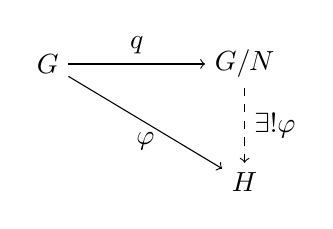
\begin{tikzpicture}
          \node (G) at (0,0) {$G$};
          \node (G/N) at (2.5,0) {$G/N$};
          \node (H) at (2.5,-1.5) {$H$};
        
\draw[->] (G) -- (G/N) node[midway, above] {$q$};
          \draw[->] (G) -- (H) node[midway, below] {$\varphi$};
          \draw[->, dashed] (G/N) -- (H) node[midway, right] {$\exists! \Bar\varphi$};

    \end{tikzpicture}
    \end{figure}
        Falls $N=\ker\varphi$ ist $\bar \varphi$ Isomorphismus siehe c)
\end{enumerate}
\end{theorem}

\begin{lemma}[Index 2 impliziert Normalität] Sei $G$ Gruppe mit $H\leqslant G$, $[G:H]=2$. Dann gilt bereits $H\triangleleft G$.
\end{lemma}
\subsection{Geometrie und Gruppen}

\begin{theorem}\Xlabel{Satz}{subsub}{von Euler} Sei $G = \mathrm{SO}(3,\R)$. Dann existiert für jedes $g\in G$ ein $l\leqslant \R^3, \dim l = 1$ mit $g\cdot l = l$ und $g$ ist eine Rotation um $l$. (Jedes Element in SO(3) ist eine Rotation und besitzt eine Rotationsachse.) Alternativ betrachte $\mathrm{SO}(3,\R)\curvearrowright \R^3$ mit $A\cdot x = Ax$, dann sagt der Satz

$$\forall g\in \mathrm{SO}(3,\R)\; \exists L\leqslant \R^3 \quad \Stab(l) = \mathrm{SO}(3,\R) \quad \forall l\in L$$
    
\end{theorem}

\begin{lemma}[Polyeder-Rotation]
    Sei $G\leqslant \mathrm{SO}(3,\R)S$ eine Gruppe, die nicht zyklisch oder isomorph zu$D_{2n}$ für $n\in \N$ ist. Dann gilt $|G|\in \{12, 24, 60\}$. Diese Zahlen erhalten wir durch \ref{Bahnformeln / Orbit-Theoreme} kombiniert mit \ref{von Euler} und der Wirkung $G\curvearrowright S^2$
\end{lemma}


\begin{theorem}\Xlabel{Satz}{subsub}{Klassifikation endlicher Rotationsgruppen}
    Sei $G\leqslant \mathrm{SO}(3,\R)$ endlich. Dann ist $G$ isomorph zu einer der folgenden Gruppen
    $$\Z/n\Z \quad D_{2n}\quad \Alt(4) \quad \Sym(4) \quad \Alt(5)$$
\end{theorem}

\subsection{Strukturtheorie}

\begin{definition}\Xlabel{Definition}{subsub}{Kurze exakte Folge / Sequenz}
Ein Diagramm von Gruppen und Homomorphismen
$$\1 \longrightarrow N \overset{i}{\longrightarrow} G \overset{q}{\longrightarrow} Q\longrightarrow \1 $$
heißt kurze exakte Folge oder \emph{k.e.S}, falls
\begin{enumerate}[label = (\roman*)]
    \item $i$ injektiv ist
    \item $q$ surjektiv ist und
    \item $\im i = \ker q$
\end{enumerate}
Falls so eine \emph{k.e.S} existiert, dann sagt man auch, dass $G$ als Erweiterung von $Q$ durch $N$ entsteht.
\end{definition}
\begin{note} Wir lösen das Problem, dass $N$ möglicherweise nicht selbst ein Normalteiler in $G$ sein kann, weil $N \not\subset G$. Mit einer k.e.S. gilt jedoch:
$$i(N) \triangleleft G$$
\end{note}

\begin{definition}[Einfach]
    Eine Gruppe $G$ (bzw. eine algebraische Struktur z.B. Ring, Modul, Algebra) heißt \emph{einfach}, falls jeder Homomorphismus $\varphi: G\to H$ entweder injektiv oder trivial ist.
\end{definition}

\begin{note}
    Eine Gruppe $G$ ist also (nach \ref{Homomorphiesatz für Gruppen}) genau dann einfach, wenn sie keine nichttrivialen Normalteiler besitzt. 
\end{note}

\begin{theorem}[Einfachheit von $\Alt(n)$] Für $n\geq 5$ ist die Gruppe $\Alt(n)$ einfach, also 
$$N \triangleleft \Alt(n) \Longleftrightarrow N = \{\1\}\; \text{ oder } \; \Alt(5)$$
\end{theorem}

\begin{note}
    Wie wir in AL20: Algebra II - Weiterführende Konzepte sehen werden, ist das der Grund, warum im Polynomring $\K[T]$ im Allgemeinen keine Lösungsformel für Gleichungen vom Grad $\geq 5$ existiert.
\end{note}

\begin{lemma}\Xlabel{Lemma}{subsub}{Erzeuger von Alt($n$)}
Die Alternierende Gruppe $\Alt(n)$ wird durch die Dreierzykel $(ijk), \; 1\leq i,j,k \leq n$ erzeugt. Für $n\geq 4$ sind je zwei Deierzykel in $\Alt(n)$ zueinander konjugiert.
\end{lemma}

\begin{definition}\Xlabel{Definition}{subsub}{Automorphismus} Ein Automorphismus $\alpha: G\to G$ ist ein invertierbarer Homomorphismus (Isomorphismus auf sich selbst). Wir bezeichnen mit $$\Aut G := \{\alpha: G\to G\; | \alpha \text{ Automorphismus}\}$$
die Gruppe der Automorphismen auf $G$ mit der Gruppenoperation $\circ$.
\end{definition}

\begin{lemma}[Innere Automorphismen, Zentrum] Die Wirkung $G\curvearrowright^C G$ ist für jedes $g\in G$ ein Automorphismus. Insbesondere gilt für jede Gruppe $G$ die Homomorphie:
$$C: G\to \Aut G, \; g\mapsto (C_g: h \mapsto ghg\r)$$
Wir bezeichnen mit $\mathrm{Inn}(G):=\im C$ die Innere Automorphismusgruppe von $G$, also alle Autormorphismen der Form $C_g$. Wir bekommen die k.e.S. nach \ref{Kurze exakte Folge / Sequenz} mit
$$\1 \longrightarrow Z(G) \longrightarrow G \longrightarrow \mathrm{Inn}(G)\overset{C}{\longrightarrow} \1$$
wobei $Z(G):= \ker C = \{ g\in G | gh = hg \; \forall h\in G\}$ das \emph{Zentrum von $G$} ist.
\end{lemma}

\begin{lemma}[Äußere Automorphismen]
Wir definieren $$\mathrm{Out}(G):= \Aut G /\mathrm{Inn}(G)$$ Es besteht die k.e.S.
$$\1 \longrightarrow \mathrm{Inn}(G) \longrightarrow \Aut G \longrightarrow \mathrm{Out}(G)\overset{q}{\longrightarrow} \1$$
\end{lemma}

\begin{definition}\Xlabel{Definition}{subsub}{Charakteristische Untergruppe} Sei $G$ eine Gruppe und $N\leqslant G$ eine Untergruppe. Dann heißt $N$ \emph{charakteristisch}, falls
$$\forall \alpha \in \Aut G \quad \alpha (N):= \{\alpha(n)| \; n\in N\} = N$$
Da insbesondere $\mathrm{Inn}(G) \subset \Aut G$ gilt
$$N \text{ charakteristisch} \Longrightarrow N \text{ normal in $G$}$$
\end{definition}

\begin{corollary}[Charakteristik $Z(G)$]
    Das Zentrum $Z(G)$ einer Gruppe $G$ ist charakteristisch.
\end{corollary}

\begin{note}[Tipp] Zur strukturtheoretischen Untersuchung der Automorphismengruppe einer Gruppe $G$ reicht es aus, Erzeuger von $G$ zu untersuchen. Die Bilder aller erzeugten Elemente sind dann durch das Bild der Erzeuger eindeutig bestimmt. Insbesondere muss Bijektivität gewährleistet sein.
\end{note}

\begin{definition}\Xlabel{Definition}{subsub}{Kommutatoruntergruppe}
Sei $G$ eine Gruppe. Dann definieren wir
$$[G,G]:=\{[x,y]|\; x,y\in G\}\qquad [x,y]:= xyx\r y\r $$
als die Kommutatoruntergruppe von $G$. Es gelten insbesondere die Relationen ($x,y,z\in G$)
\begin{enumerate}[label=\roman*)]
    \item $[x,y]\r = [y,x]$
    \item $[xy,z] = x[y,z]x\r [x,z] =: [y^x, z^x]$
    \item $[z,xy] = [z,x]x[z,y]x\r = [z,x][z^x, y^x]$
\end{enumerate}
\end{definition}

\begin{corollary}[Charakteristik Kommutatoruntergruppe]
Die Kommutatoruntergruppe $[G,G]$ von $G$ ist charakteristisch. Insbesondere ist der Quotient $G_{ab} := G/[G,G]$ eine abelsche Gruppe genannt Ableanisierung von $G$ die die universelle Eigenschaft erfüllt analog zu \ref{Homomorphiesatz für Gruppen} d).
\end{corollary}

\begin{note}
    Falls $G$ abelsch, dann ist $[G,G] =\{\1\}$ und $G_{ab} = G$
\end{note}

\begin{definition}\Xlabel{Definition}{subsub}{Derivierte Reihe}
Sei $(G^{(k)})_{k\in \N}$ rekursiv definiert durch:
$$G^{(0)} := G,\qquad G^{(k)}:= [G^{(k-1)},G^{(k-1)}], \; k\geq 1$$
Wir bezeichnen $(G^{(k)})_{k\in \N}$ als die derivierte Reihe von $G$. Insbesondere gilt in absteigender Weise:
$$...\triangleright G^{(k-1)} \triangleright G^{(k)} \triangleright G^{(k+1)} \triangleright ... $$
(eigentlich sogar mehr, nämlich Charakteristik)
\end{definition}

\begin{note}
    Obwohl nicht gleich offensichtlich, gelt jedoch ebenso auch $G^{(k)} \triangleleft G$
\end{note}

\begin{definition}\Xlabel{Definition}{subsub}{Auflösbarkeit}
    Eine Gruppe $G$ heißt \emph{auflösbar}, wenn ihre derivierte Reihe an $\1$ stabilisiert, also
    $$G^{(k)}\overset{n\to \infty}{\longrightarrow} \{\1\}$$
\end{definition}

\begin{note}\mbox{}
    \begin{enumerate}[label= -]
        \item Abelsche Gruppen sind auflösbar und stabilisieren bereits nach einem Schritt in der derivierten Reihe.
        \item Eine einfache nicht-abelsche Gruppe kann nicht auflösbar sein, weil ansonsten ein nicht-trivialer Normalteiler existieren würde.
    \end{enumerate}
\end{note}

\begin{lemma}\Xlabel{Lemma}{subsub}{Auflösbarkeit Untergruppe und Quotient} Sei $G$ eine auflösbare Gruppe, dann gilt für jede Quotientenabbildung $q:G\to Q$ und jede Untergruppe $H\leqslant G$:
$$H \text{ ist auflösbar} \quad \& \quad Q \text{ ist auflösbar} $$
\end{lemma}

\begin{theorem}\Xlabel{Satz}{subsub}{Auflösbarkeit in einer k.e.S.} Sei eine k.e.S. gegeben durch
$$\1 \longrightarrow N \overset{i}{\longrightarrow} G \overset{q}{\longrightarrow} Q\longrightarrow \1 $$
Dann gilt:
$$N, Q \text{ sind auflösbar } \Longleftrightarrow \;  G \text{ ist auflösbar}$$
    
\end{theorem}

\begin{note}
    Satz \ref{Auflösbarkeit in einer k.e.S.} ist fundamental zur Untersuchung von endlichen Gruppen. Dieser Satz ermöglicht es schlussendlich die Struktur endlicher Gruppen zu klassifizieren und auf die Bestandteile $N$ und $Q$
\end{note}

\begin{definition}\Xlabel{Definition}{subsub}{Normalreihe}
    Sei $G$ eine Gruppe. Eine absteigende Folge $(N_k)_{k\in \N} \triangleleft G$ von Normalteilern in $G$ heißt Normalreihe. Wir nennen $(N_k)_{k\in \N}$ endlich, falls für 
    $$G\supset N_1 ...\supset N_k \supset ...$$
    ein $n\in \N$ existiert, sodass $N_{l}= \{\1\}$ für $l\geq n$. Wir bezeichnen $N_k/N_{k+1}$ als die Subquotienten der Normalreihe.
\end{definition}

\begin{note} Die derivierte Reihe $G^{(k)}$ ist solch eine Normalreihe mit abelschen Subquotienten. Wir benötigen diesen etwas allgemeineren Begriff, weil für die nachfolgende Eigenschaft eine Äquivalenz gilt. \end{note}

\begin{theorem}\Xlabel{Satz}{subsub}{Auflösbarkeit und Normalreihe}
Eine Gruppe $G$ ist genau dann auflösbar, wenn sie eine Normalreihe $(N_k)_{k\in \N}\triangleleft G$ mit abelschen Subquotienten besitzt.
\end{theorem}

\begin{note} Die Äquivalenz \ref{Auflösbarkeit und Normalreihe} gibt uns zumindest die Möglichkeit direkt zu sagen, ob eine Gruppe auflösbar ist, wenn wir irgendeine Normalreihe von $G$ mit abelschen Subquotienten bereits kennen. In jeglich sonstiger Hinsicht ist die Aussage eher schwach.\end{note}

\begin{definition}[Untere Zentralreihe] Sei $G$ eine Gruppe. Dann definieren wir die Folge $(G_{(k)})_{k\in\N} = (\gamma_k(G))_{k\in\N}$ rekursiv durch
$$\gamma_0(G) := G \qquad \gamma_{k}(G) = [G,\gamma_{k-1}(G)]$$
Diese heißt untere Zentralreihe an $G$. Wir nennen eine Normalreihe aus \ref{Normalreihe} auch Zentralreihe, falls die Subquotienten $N_k/N_{k+1}$ überdies zentral in $G/N_{k+1}$ sind.
\end{definition}

\begin{definition}\Xlabel{Definition}{subsub}{Nilpotenz}
Eine Gruppe $G$ heißt nilpotent, wenn ihre untere Zentralreihe an $\{\1\}$ stabilisiert. 

\end{definition}

\begin{note}
Jede nilpotente Gruppe ist auflösbar, weil die Subquotienten offensichtlich abelsch sind. Die Umkehrung gilt jedoch nicht. In der Situation von \ref{Auflösbarkeit in einer k.e.S.} ist $G$ außerdem nilpotent, wenn $N$ und $Q$ nilpotent sind und außerdem $N\leqslant Z(G)$.
\end{note}


\subsection{Sylow-Theorie}

\begin{definition}\Xlabel{Definition}{subsub}{p-Gruppe} Sei $G$ eine Gruppe mit $|G|=p^n$ für $p$ \emph{prim} und $n\in \N$. Dann nennen wir $G$ eine $p-$Gruppe.
\end{definition}

\begin{lemma}[Eigenschaften von $p-$Gruppen] Sei $G$ eine $p-$Gruppe. Dann gilt
\begin{enumerate}
\item Falls $G\neq \{\1\}$ dann ist $Z(G)\neq \{\1\}$
\item $G$ ist nilpotent
\item Falls $|G|=p^2$, dann ist $G$ abelsch.
\end{enumerate}
\end{lemma}

\begin{definition}\Xlabel{Definition}{subsub}{p-Sylow-Untergruppe}
Sei $G$ eine Gruppe und $|G|= m\cdot p^n$ für $m,n\in \N, p$ \emph{prim} und $\gcd(m,p)=1$. (Eine solche Darstellung gibt es immer.) Dann heißt $S\leqslant G$ eine \emph{$p-$Sylow-Untergruppe}, falls $|S|=p^n$. Wir bezeichnen mit
$$\Syl_p(G):=\{S\leqslant G| \; S \text{ ist $p-$Sylow-Untergruppe}\}$$
die Menge der $p-$Sylow-Untergruppen von $G$. Im Nachfolgenden nennen wir diese Art von Untergruppen der Einfachheit halber gelegentlich $p-$Sylow's.

\end{definition}

\begin{theorem}\Xlabel{Satz}{subsub}{Erster Sylow-Satz}
Sei $G$ endlich. Für jede Primzahl $p|\; |G|$ existiert eine $p-$Sylow-Untergruppe.
\end{theorem}

\begin{theorem}\Xlabel{Satz}{subsub}{Zweiter Sylow-Satz} Sei $G$ eine endliche Gruppe und $p$ \emph{prim}. Dann gilt
\begin{enumerate}[label = \roman*)]
    \item Jede $p-$Untergruppe ist in einer $p-$Sylowuntergruppe enthalten
    \item Alle $p-$Sylows sind zueinander konjugiert, also 
    $$\forall g \in G \quad g\Syl_p(G)g\r = \Syl_p(G)$$
\end{enumerate}

\end{theorem}

\begin{corollary}[Normalität durch Sylow] Sei $G$ eine Gruppe und $S\leqslant G$ die einzige $p-$Sylowuntergruppe. Dann ist $S\triangleleft G$ und $G$ nicht einfach.   
\end{corollary}

\begin{theorem}\Xlabel{Satz}{subsub}{Dritter Sylow-Satz}
Sei $G$ eine endliche Gruppe und $p$ \emph{prim}. Dann ist
$$|\Syl_p(G)| \equiv 1 \mod p$$
\end{theorem}

\subsection{Semidirekte Produkte}

\begin{definition}[Semidirektes Produkt]
    Sei eine Wirkung $H\curvearrowright^\alpha \Aut N$ gegeben. Dann definiere $N\rtimes_\alpha H$ als diejenige Gruppe der Obermenge $N\times H$ mit der Gruppenoperation
    $$(n_1, h_1)(n_2, h_2) := (n_1\alpha_{h_1}(n_2), h_1h_2) \qquad (n,h)\r:=(\alpha_{h\r}(n\r),h\r)$$
    Die Gruppe $N\rtimes_\alpha H$ heißt \emph{semidirektes Produkt} von $N$ und $H$ bezüglich der Wirkung $\alpha:H \to \Aut N$
\end{definition}

\begin{note}
    Die Gruppe $N\rtimes_\alpha H$ enthält die Gruppen
    $$N\cong \{(n,\1)|\; n\in N\} \triangleleft N\rtimes_\alpha H \qquad H\cong \{(\1,h)|\; h\in H\}\leqslant N\rtimes_\alpha H$$
    Wir bekommen entsprechend als k.e.S.
    $$\1 \longrightarrow N \overset{i}{\longrightarrow} N \rtimes_\alpha H \overset{q}{\longrightarrow} H \longrightarrow \1$$
    mit $i(n)=(n,1)$ und $q(n,h)=h$ mit einer Besonderheit
\end{note}

\begin{definition}\Xlabel{Definition}{subsub}{Spaltung}
Eine kurze exakte Folge $$\1 \longrightarrow N \overset{i}{\longrightarrow} G \overset{q}{\longrightarrow} Q\longrightarrow \1 $$
\emph{spaltet}, falls ein Homomorphiusmus $s:Q \to G$ existiert mit $q\circ s = \id_Q$. Wir können dann `` $Q$ aus $G$ herausschneiden''
\end{definition}

\begin{note}
    Eine kurze exakte Folge 
    $$\1 \longrightarrow N \overset{i}{\longrightarrow} N \rtimes_\alpha H \overset{q}{\longrightarrow} H \longrightarrow \1$$
    spaltet.
\end{note}

\begin{theorem}\Xlabel{Satz}{subsub}{Semidirekte Produkte und Spaltende Erweiterungen}
Es gilt die folgende Äquivalenz
$$\1 \longrightarrow N \overset{i}{\longrightarrow} G \overset{q}{\longrightarrow} Q\longrightarrow \1  \text{ spaltet} \quad\Longleftrightarrow\quad  G \cong N\rtimes_\alpha Q$$
    
\end{theorem}

\begin{theorem}[Anwendung: Gruppen oder Ordnung 12] Sei $|G|=12$. Dann ist $G$ isomorph zu einer der folgenden Gruppen
$$\Z/12\Z\qquad \Z/2\Z \times \Z/6\Z \qquad D_{12} \qquad \Alt(4) \qquad \mathrm{Dic}_3$$
    
\end{theorem}
\subsection{Erzeuger und Relationen}

\begin{definition}\Xlabel{Definition}{subsub}{Wort}
Sei $A$ eine Menge. Ein Wort $w$ mit Buchstaben in $A$ ist eine endliche Folge $a_1a_2\cdots a_n$ mit $a_i\in A, \; (n\in \N)$. Die Menge der Wörter mit Buchstaben in $A$ wird mit $A^* $ bezeichnet.
\end{definition}

\begin{definition}[Produkt von Wörtern] \label{Produkt von Wörtern}Seien $w,w'$ zwei Wörter mit Buchstaben in $A$. 
$$w=a_1 \cdots a_n \qquad w' = a_1'\cdots a_m'$$
Das Produkt $ww'$ wird definiert als
$$ww'=a_1 \cdots a_n a_1'\cdots a_m'$$
\end{definition}

\begin{definition}[Menge der reduzierten Wörter] Sei $S$ Menge und setze $\bar S:\{\bar s| \; s\in S\}$ sowie $A:=S\sqcup \bar S$. Wir definieren die Menge der reduzierten Wörter 
$$\mathbf{F}_S := \{w\in A^*| \; \text{ für jedes $s\in S$ enthält w kein Teilwort der Gestalt $s\bar s$ oder $\bar s s$}\} $$
Falls $w\in A^* \setminus \mathbf F _S$, dann heißt $w$ reduzibel. Eine Reduktion eines reduziblen Worts ist das schrittweise entfernen von Teilwörtern der Form $s\bar s$ bzw. $\bar s s $. Diese Operation nennen wir $\mathrm{Red}(w)$
\end{definition}
\begin{definition}\Xlabel{Definition}{subsub}{Freie Gruppe} Wir bezeichnen $\mathbf{F}_S$ als die freie Gruppe über der Erzeugendenmenge $S$ mit der Gruppenoperation
$$w\cdot w:= \mathrm{Red}(ww')$$
mit $ww'$ im Sinne von \ref{Produkt von Wörtern}. Diese ist tatsächlich assoziativ mit Existenz von Neutralem und Inversen Element(en).
    
\end{definition}

\begin{lemma}[Universelle Eigenschaft der freien Gruppe] Als Alternativdefinition oder auch als Eigenschaft sagen wir: Eine Gruppe $F_S$ heißt frei auf der erzeugenden Menge $S$, wenn 
\begin{enumerate}[label=\roman*)]
    \item $S\subset F_S$
    \item für jede Gruppe $G$ und für jede Abbildung $\varphi: S\to G$ existiert ein eindeutiger Homomorphismus $\bar \varphi: F_s\to G $ mit $\bar \varphi | _S = \varphi$. Es gilt wieder das kommutative Diagramm
\end{enumerate}

\begin{figure}[h]
        \centering
    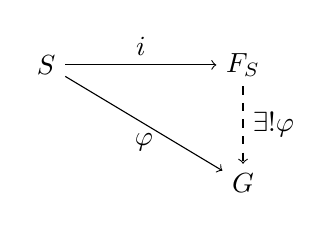
\begin{tikzpicture}
          \node (S) at (0,0) {$S$};
          \node (FS) at (2.5,0) {$F_S$};
          \node (G) at (2.5,-1.5) {$G$};
        
\draw[->] (S) -- (FS) node[midway, above] {$i$};
          \draw[->] (S) -- (G) node[midway, below] {$\varphi$};
          \draw[->, dashed] (FS) -- (G) node[midway, right] {$\exists! \Bar\varphi$};

    \end{tikzpicture}
    \end{figure}
    Tatsächlich ist $\mathbf{F}_S$ die eindeutige freie Gruppe mit genau dieser universellen Eigenschaft.
\end{lemma}

\begin{definition}[Freie Gruppe vom Rang n] Die Gruppe $\mathbf{F}_n= \mathbf F_{\langle s_1, ...., s_n\rangle}$ heißt freie Gruppe vom Rang $n$ oder auf $n$ Erzeugern.    
\end{definition}

\begin{lemma}[Relation zwischen Gruppen und freien Gruppen] Sei $G$ eine Gruppe. Dann gilt
\begin{enumerate}
    \item $G$ ist Quotient einer freien Gruppe.
    \item Falls $G=\langle g_1, ..., g_n\rangle$, dann ist $G$ sogar ein Quotient einer freien Gruppe $\mathbf{F}_n$v vom Rang $n$
\end{enumerate}
    
\end{lemma}

\begin{definition}\Xlabel{Definition}{subsub}{Normale Hülle} Sei $G$ eine Gruppe und $R\subset G$ eine Teilmenge. Dann nennen wir 
$$\langle\!\langle R \rangle\!\rangle := \bigcap_{R\subset N \triangleleft G} N$$
die normale Hülle in $R$. Analog zu \ref{Erzeugte Untergruppen} ist $N$ der kleinste Normalteiler in $G$, der $R$ enthält.
    
\end{definition}

\begin{definition}\Xlabel{Definition}{subsub}{Universelle Gruppe} Sei $S$ eine Menge (Menge der Erzeuger) und $R\subset \mathbf F_S$ eine Teilmenge (Menge der Relationen). Die Gruppe 
$$\langle S| R\rangle := \mathbf{F}_S / \langle\!\langle R \rangle\!\rangle $$ heißt universelle Gruppe erzeugt durch $S$ mit Relationen $R$. Falls $G\cong \langle S| R\rangle$, so sagt man, dass $G$ eine Präsentation mit Erzeugern $S$ und Relationen $R$ besitzt.
    
\end{definition}
\newpage
\begin{note} Diese Theorie hilft uns, beliebige Gruppen mit Präsentation durch Erzeuger und Relationen in Garphen, soganannten \emph{Cayley-Graphen} zu untersuchen. Ein Beispiel sei gezeigt für die folgenden Gruppen. 
    

\begin{figure}[h] 
 \centering 
   \begin{subfigure}[b]{0.45\linewidth}
   \centering
   \resizebox{\linewidth}{!}{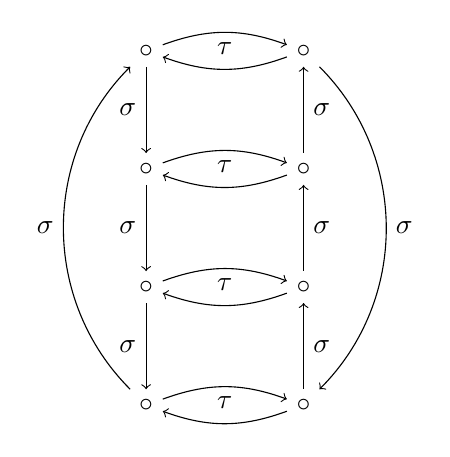
\begin{tikzpicture}
        \node (r1) at (0,0) {$\circ$};
        \node (r2) at (0,-1.5) {$\circ$};
        \node (r3) at (0,-3) {$\circ$};
        \node (r4) at (0,-4.5) {$\circ$};

        \node (rm1) at (2,0) {$\circ$};
        \node (rm2) at (2,-1.5){$\circ$};
        \node (rm3) at (2,-3) {$\circ$};
        \node (rm4) at( 2,-4.5){$\circ$};

        \draw[->] (r1)--(r2) node[midway, left] {$\sigma$};
        \draw[->] (r2)--(r3) node[midway, left] {$\sigma$};
        \draw[->] (r3)--(r4) node[midway, left] {$\sigma$};
        \draw[->, bend left = 45] (r4) to node[midway, left] {$\sigma$} (r1) ;

        \draw[<-] (rm1)--(rm2) node[midway, right] {$\sigma$};
        \draw[<-] (rm2)--(rm3) node[midway, right] {$\sigma$};
        \draw[<-] (rm3)--(rm4) node[midway, right] {$\sigma$};
        \draw[<-, bend right = 45] (rm4) to node[midway, right] {$\sigma$} (rm1);

        \draw[->, bend left=20] (r1) to node[midway, below] {$\tau$} (rm1) ;
        \draw[->, bend left=20] (rm1) to (r1) ;
        \draw[->, bend left=20] (r2) to node[midway, below] {$\tau$} (rm2) ;
        \draw[->, bend left=20] (rm2) to (r2) ;
        \draw[->, bend left=20] (r3) to node[midway, below] {$\tau$} (rm3) ;
        \draw[->, bend left=20] (rm3) to (r3) ;
        \draw[->, bend left=20] (r4) to node[midway, below] {$\tau$} (rm4) ;
        \draw[->, bend left=20] (rm4) to (r4) ;
         \end{tikzpicture}
         }
        \caption*{\centering $D_8$ mit Präsentation \par $\langle \sigma, \tau \;|\; \sigma^4 = \id, \; \tau^2 = \id, \sigma\tau\sigma = \tau\rangle$}
         \end{subfigure}
         \hfill
        \begin{subfigure}[b]{0.45\linewidth}
        \centering
        \resizebox{\linewidth}{!}{\begin{tikzpicture}
            \node (A) at (0,0) {$\circ$};
            \node (B) at (0,-1.5) {$\circ$};
            \node (C) at (0,-3) {$\circ$};
            \node (D) at (1.5,0) {$\circ$};
            \node (E) at (1.5,-1.5) {$\circ$};
            \node (F) at (1.5,-3) {$\circ$};
            \node (G) at (3,0) {$\circ$};
            \node (H) at (3,-1.5) {$\circ$};
            \node (I) at (3,-3) {$\circ$};
            
            \node (AAU) at (0,1.5) {$\vdots$};
            \node (AA) at (-1.5,0) {$\hdots$};
            \node (BB) at (-1.5,-1.5) {$\hdots$};
            \node (CC) at (-1.5,-3) {$\hdots$};
            \node (CCD) at (0,-4.5) {$\vdots$};
            
            \node (GGU) at (3,1.5) {$\vdots$};
            \node (GG) at (4.5,0) {$\hdots$};
            \node (HH) at (4.5,-1.5) {$\hdots$};
            \node (II) at (4.5,-3) {$\hdots$};
            \node (IID) at (3,-4.5) {$\vdots$};
            
            \node (DDU) at (1.5,1.5) {$\vdots$};
            \node (FFD) at (1.5,-4.5) {$\vdots$};
            
            \draw[->] (AAU)--(A) node[midway, left] {$t$};
            \draw[->] (A)--(B) node[midway, left] {$t$};
            \draw[->] (B)--(C) node[midway, left] {$t$};
            \draw[->] (C)--(CCD) node[midway, left] {$t$};

            \draw[->] (DDU)--(D) node[midway, left] {$t$};
            \draw[->] (D)--(E) node[midway, left] {$t$};
            \draw[->] (E)--(F) node[midway, left] {$t$};
            \draw[->] (F)--(FFD) node[midway, left] {$t$};

            \draw[->] (GGU)--(G) node[midway, left] {$t$};
            \draw[->] (G)--(H) node[midway, left] {$t$};
            \draw[->] (H)--(I) node[midway, left] {$t$};
            \draw[->] (I)--(IID) node[midway, left] {$t$};

            \draw[->] (AA)--(A) node[midway, above] {$s$};
            \draw[->] (A)--(D) node[midway, above] {$s$};
            \draw[->] (D)--(G) node[midway, above] {$s$};
            \draw[->] (G)--(GG) node[midway, above] {$s$};

            \draw[->] (BB)--(B) node[midway, above] {$s$};
            \draw[->] (B)--(E) node[midway, above] {$s$};
            \draw[->] (E)--(H) node[midway, above] {$s$};
            \draw[->] (H)--(HH) node[midway, above] {$s$};

            \draw[->] (CC)--(C) node[midway, above] {$s$};
            \draw[->] (C)--(F) node[midway, above] {$s$};
            \draw[->] (F)--(I) node[midway, above] {$s$};
            \draw[->] (I)--(II) node[midway, above] {$s$};
            
        \end{tikzpicture}
        }
        \caption*{$\Z^2$ mit Präsentation $\langle s,t\; |\; st = ts\rangle $}
    \end{subfigure}

\end{figure}


Die Knoten innerhalb eines Caley-Graphen stehen für die Elemente der Gruppe und die Pfeile oder Verbindungen für die Relation zwischen ihnen.
\end{note}

\PropertyNotice

\end{document}